\documentclass[10pt]{article}

\usepackage{polski}
\usepackage{graphicx}
\usepackage{hyperref}
\graphicspath{{images/}}

\usepackage{geometry}
\newgeometry{tmargin=4cm, bmargin=4cm, lmargin=3.2cm, rmargin=3.2cm}

\usepackage{fancyhdr}
\pagestyle{fancy}

\usepackage{float}



\begin{document}

\begin{titlepage}


\begin{center}

  \LARGE \textsc{Politechnika Wrocławska}\\
  \vspace*{0.2cm}
  \Large \textsc{Wydział Informatyki i Telekomunikacji}\\
  \vspace*{0.4cm}
  \centering
\includegraphics[width=0.2\textwidth]{WITlogo.png}\\
  \vspace*{0.2cm}
  \vspace*{2cm}

  \centerline{\rule{\textwidth}{1.2pt}}
  \vspace{0.4cm}
  \Huge\textbf{Metody i Systemy Decyzyjne}
  \centerline{\rule{\textwidth}{1.2pt}}
  \vspace{1cm}
  \LARGE Sprawozdanie z laboratorium\\
  \vspace{3.5cm}
  \textsc{Autor}\\
  \vspace{0.2cm}
  \textbf{Dariusz Majnert}\\
  \vspace{0.1cm}
  \Large nr albumu: \textbf{272748}\\
  \vspace{0.1cm}
  kierunek: \textbf{Informatyka Stosowana}

  \vspace*{\fill}
  \Large \textit{\today}

 \end{center}


\end{titlepage}


\begin{abstract}
Celem pracy jest stworzenia estymatora kosztu wynajmu mieszkania na podstawie danych uzyskanych z serwisu ogłoszeniowego. 
\textbf{Do stworzenia estymatora wykorzystanko regresję liniową} z danych które zostały przeanalizowane pod kątem największego wpływu na koszt wynajmu.
\end{abstract}

\section{Wstęp -- sformułowanie problemu}
\label{sec:wstep}

Rynek mieszkaniowy w Polsce jest dynamiczny i złożony, a jego kondycja jest ściśle powiązana z ogólną sytuacją gospodarczą, polityką mieszkaniową państwa, a także czynnikami demograficznymi i społecznymi. 
Duże miasta charakteryzują się dużym popytem na mieszkania, co może prowadzić do windowania cen, a potencjalni najemcy chcą podjąć decyzje o wynajmie świadomie i w oparciu o dokładne informacje.

Celem raportu jest analiza tego, co najbardziej wpływa na cenę wynajmu mieszkania we Wrocławiu, a następnie stworzenie estymatora kosztu wynajmu mieszkania na podstawie tych danych.


\section{Opis rozwiązania}

\subsection{Pozyskiwanie danych}
\subsubsection{Pobieranie danych o mieszkaniach}
Dane ofert wynajmu mieszkania były zbierane z niepublicznego API serwisu OLX, wykorzystywanego przez stronę internetową portalu, w okresie od 08.05.2024 do 01.06.2024 przez skrypt pobierający dane, który uruchamiany był co godzinę i pobierał 1000 najnowszych ofert we Wrocławiu.

W celu usunięcia redundantych danych, powstałych przez częste zapisywanie zestawu danych, wykorzystany został identyfikator zapisany w każdym ogłoszeniu, który umożliwił jednoznaczną identyfikacje i zapisanie tylko jednej kopii.

Zestaw danych zawiera tytuł i opis ogłoszenia, a także informacje o cenie wynajmu, czynszu, metrażu mieszkania, typie zabudowy, liczbie pokojów i piętrze na którym znajduje się mieszkanie.

\subsubsection{Ekstrakcja adresu mieszkania}

W ofertach zwracanych przez API nie było bezpośredniego sposobu, aby odczytać dokładną lokalizację mieszkania, dlatego użyty został model językowy OpenAI ChatGPT (gpt-3.5-turbo-0125) w celu ekstrakcji adresu wykorzystując tytuł i opis ogłoszenia.


Poleceniem systemowym dla modelu było:
\begin{verbatim}
Twoim zadaniem jest wyciągnąć adres mieszkania z przekazanych
danych dotyczących oferty wynajmu mieszkania we Wrocławiu. 
Odpowiadaj w formacie JSON w formie { "address":  } . 
Bądź zwięzły i jeżeli nie znajdziesz informacji o adresie to daj null.
\end{verbatim}

W procesie ekstrakcji z zestawu danych odrzucone zostały informacje o tytule i opisie ogłoszenia, natomiast dodany został adres mieszkania. 
Ogłoszenia dla których nie udało się wyekstraktować adresu zostały odrzucone.

\subsubsection{Geokodowanie adresu mieszkania}
Aby móc jednoznacznie określić położenie mieszkania, wykorzystane zostało API Google Maps, a dokładniej usługa Geocoding API. 
Dla każdego ogłoszenia zostało wysłane zapytanie do API z adresem wyekstrahowanym przez model językowy. 
W przypadku braku nazwy miasta w adresie, dodawany zostawał sufiks ``\textit{, Wrocław}".

Wartościami zwracanymi z interfejsu były współrzędne geograficzne w formacie stopni w zapisie dziesiętnym (DD). 
Do zestawu danych, dla mieszkań dla których udało się określić współrzędne, dodane zostały długość i szerokość geograficzna mieszkania. 
W przypadku nieudanego geokodowania ogłoszenie było odrzucane.  

\subsubsection{Wyjściowy zestaw danych}
Wyjściowy zestaw danych zawiera informacje o cenie wynajmu, czynszu, metrażu mieszkania, typie zabudowy, liczbie pokojów, 
piętrze na którym znajduje się mieszkanie, adresie i współrzędnych geograficznych mieszkania. 
Do każdej oferty zapisany jest identyfikator ogłoszenia z portalu OLX.

Po niecałym miesiącu zbierania danych, po transformacjach, zestaw zawiera informacje o $ 4058 $ ofertach wynajmu mieszkania, które zostały zapisane w formacie CSV. 


\subsection{Wstępna analiza danych}
Wstępnie zostało nakreślone kilka wykresów dla ceny, powierzchni, położenia mieszkań i rodzaju zabudowy w celu ocenienia jakości zgromadzonych danych. 
Wykresy te wykazują zanieczyszczenie danych, na co wskazują 

\begin{itemize}
    \item Mieszkania o zbyt wysokiej lub nierealnie niskiej cenie
    \item Mieszkania o zbyt dużej powierzchni
    \item Położenie geograficzne nie na terenie miasta Wrocław
\end{itemize}


\begin{figure}[H]
    \centering
    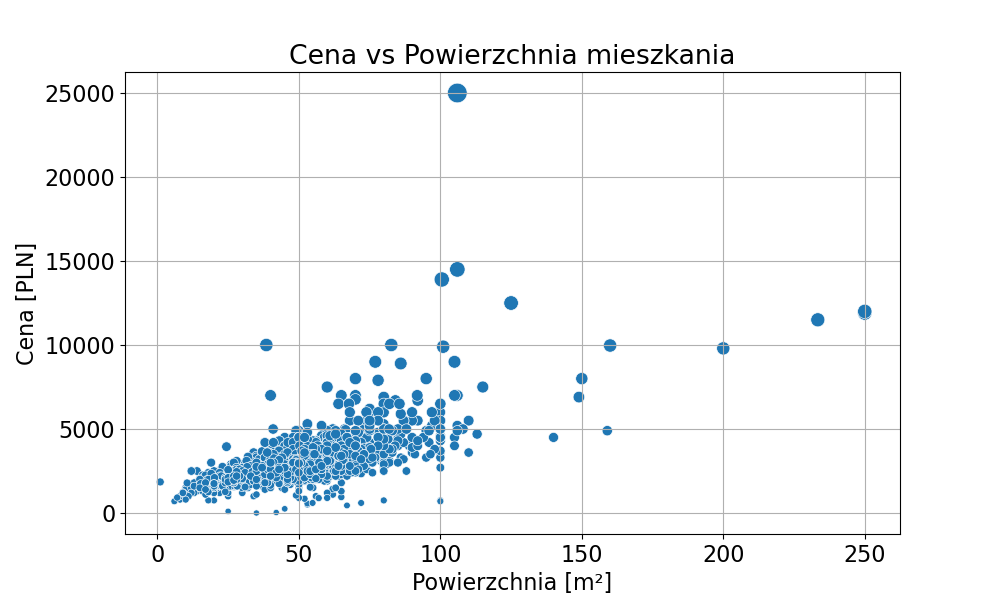
\includegraphics[width=0.6\linewidth]{prices-area-unfiltered.png}
    \caption{Wykres rozrzutu ceny i powierzchni mieszkania przed filtrowaniem}
    \label{fig:prices_area_unfiltered}
\end{figure}

\begin{figure}[H]
    \centering
    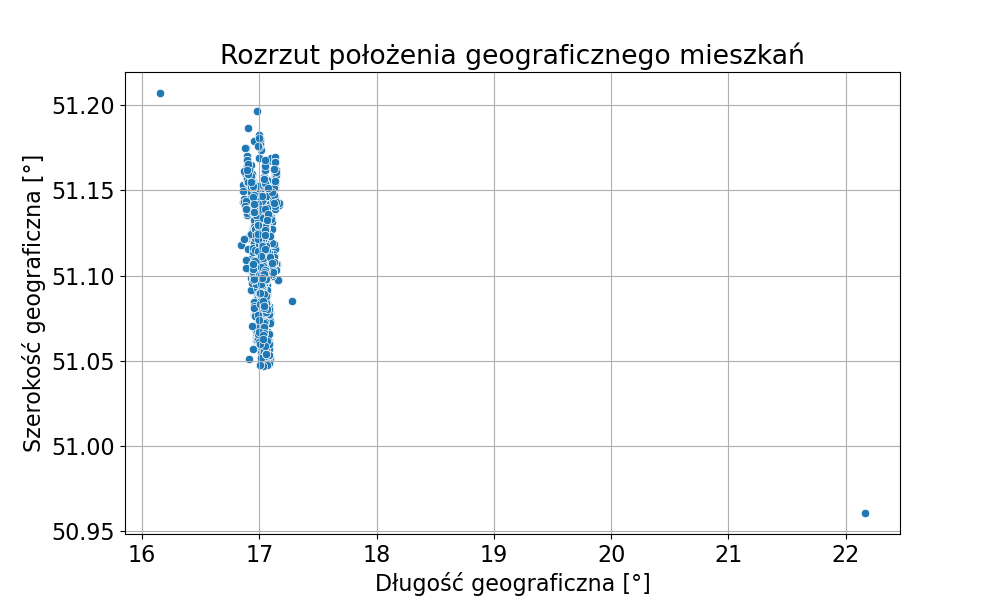
\includegraphics[width=0.6\textwidth]{location-unfiltered.png}
    \caption{Wykres rozrzutu położenia geograficznego mieszkania przed filtrowaniem}
    \label{fig:location_unfiltered}
\end{figure}

\begin{figure}[H]
    \centering
    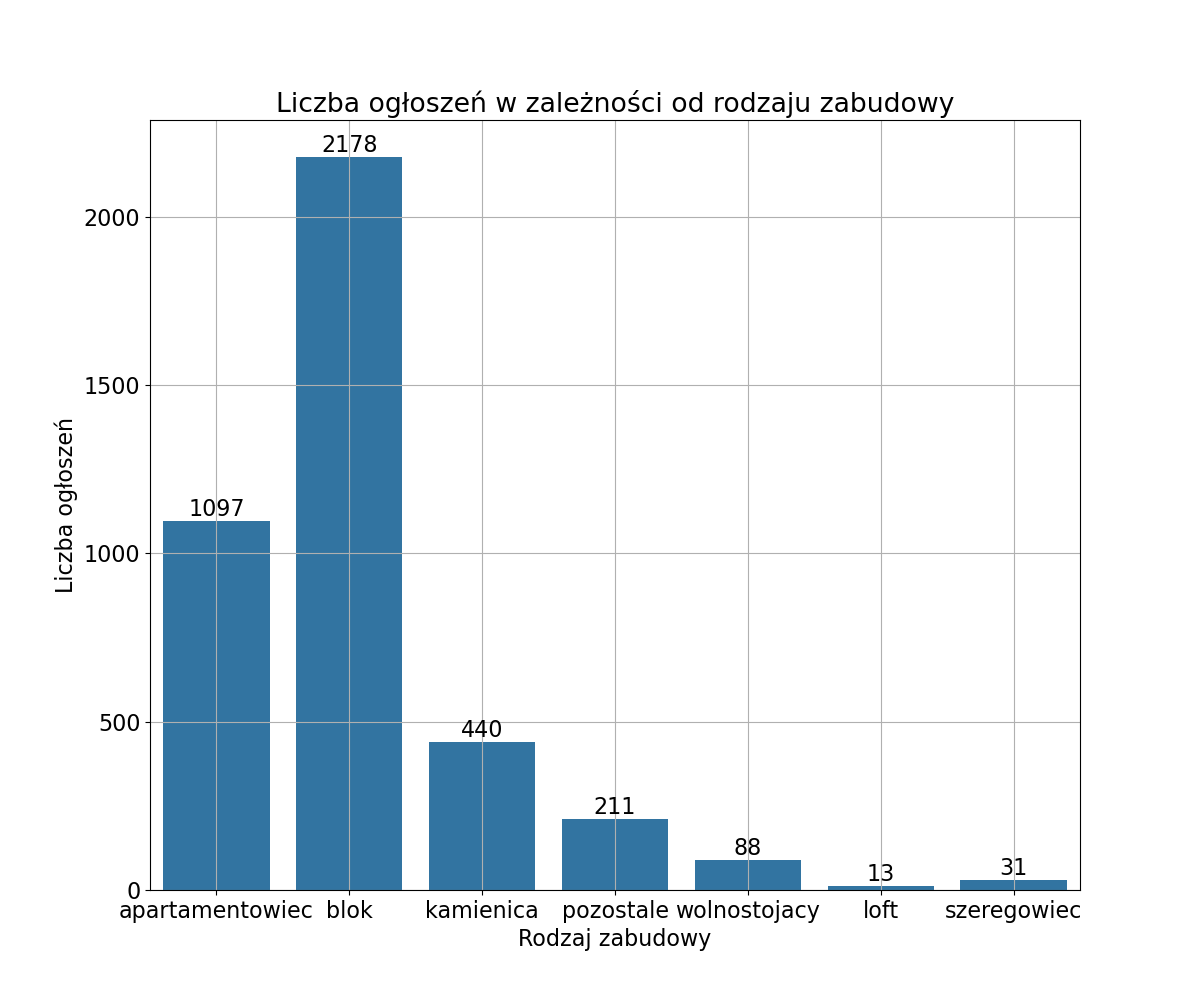
\includegraphics[width=0.6\textwidth]{builttype-count-unfiltered.png}
    \caption{Wykres liczby mieszkań ze względu na rodzaj zabudowy}
    \label{fig:builttype_count_unfiltered}
\end{figure}

\subsection{Filtrowanie danych}
Dane zostały przefiltrowane tak, aby odrzucić wartości skrajne według następujących reguł

\begin{itemize}
    \item $ 1000 \leq $ Cena wynajmu $ < 10000 $
    \item $ 5m^2 \leq $ Powierzchnia $ < 125m^2 $
    \item $ 51.04 \leq $ Szerokość geograficzna $ \leq 51.19 $
    \item $ 16.83 \leq $ Długość geograficzna  $ \leq 17.19 $
    \item Mieszkanie musi być umeblowane
\end{itemize}



\subsection{Eksploracja danych}
Celem badania jest określenie parametrów w zestawie danych które wpływają na cene wynajmu mieszkania we Wrocławiu, a następnie na ich podstawie spróbować oszacować cenę wynajmu mieszkania.

\subsubsection{Metraż mieszkania}

Przy wstępnej analizie danych można było zauważyć na rysunku \ref{fig:prices_area_unfiltered}, że powierzchnia mieszkania ma znaczący wpływ na jego cenę, co dalej potwierdza ich współczynnik korelacji Pearsona równy $ 0.70 $. 

\subsubsection{Liczba pokojów}

Dla liczby pokojów można zauważyć silną korelację z ceną mieszkania, natomiast ta charakterystyka silnie koreluje z powierzchnią mieszkania (współcznnik korelacji $ 0.76 $), dlatego postanowiono nie brać jej pod uwagę.

\begin{figure}[H]
    \centering
    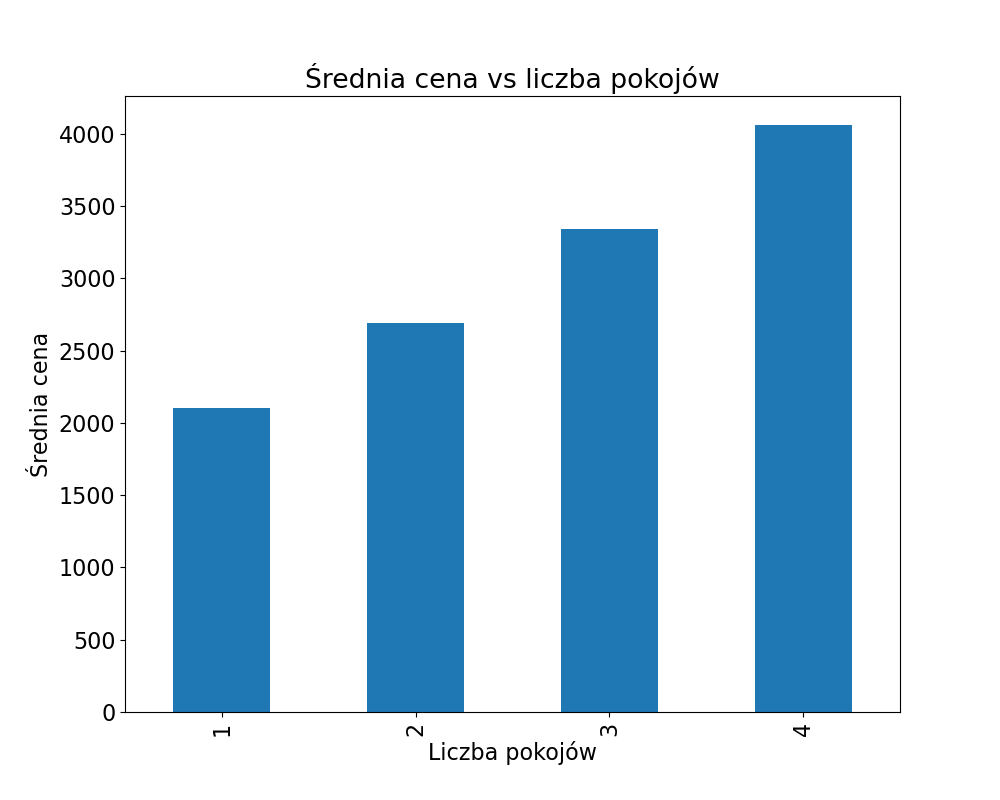
\includegraphics[width=0.6\textwidth]{room-count-price.png}
    \caption{Wykres liczby pokojów i średnia cena wynajmu mieszkania}
    \label{fig:room_count_price}
\end{figure}

\subsubsection{Czynsz}

Z uwagi na niepełne informacje na temat czynszu w niektórych ofertach, nie brano go pod uwagę jako potencjalna charakterystyka. 
Dodatkowo analiza korelacji wskazała, że czynsz jest bardziej skorelowany z powierzchnią mieszkania niż z samą ceną wynajmu (współczynnik wyniósł odpowiednio $0.40 $ i $ 0.32 $).

\subsubsection{Rodzaj zabudowy}

Ze względu na małą liczbę danych dotyczących budynków w zabudowie typu ``wolnostojacy", ``loft" i ``szeregowiec", zostały one zgeneralizowane do kategorii ``pozostale".
Po takiej zmianie, został nakreślony wykres średniej ceny mieszkania w zależności od rodzaju zabudowy. Zauważalna jest znaczna różnica w cenie pomiędzy nimi, dlatego charakterystyka ta będzie brana pod uwagę przy oszacowaniu ceny.

\begin{figure}[H]
    \centering
    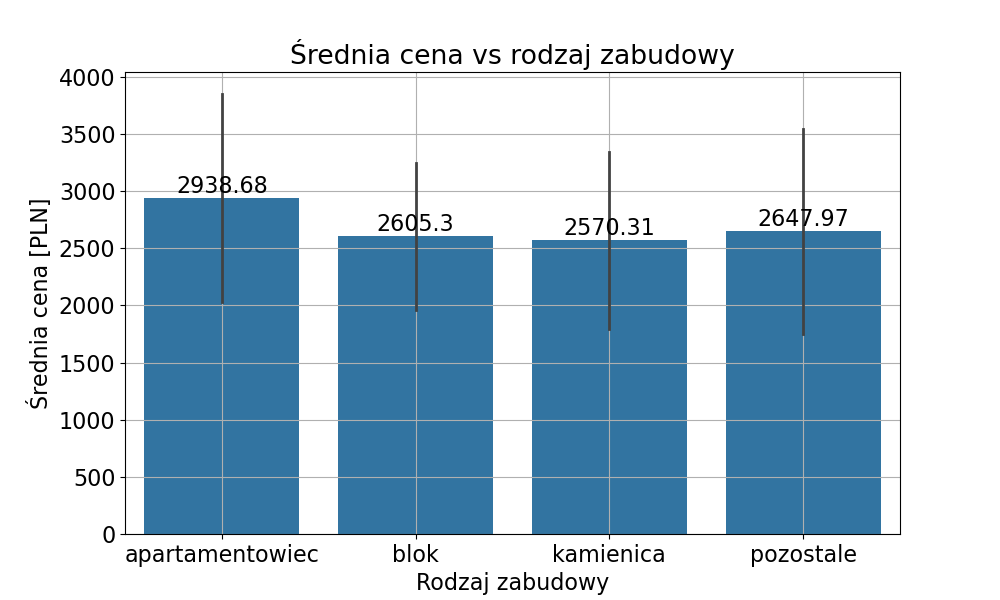
\includegraphics[width=0.6\textwidth]{builttype-price.png}
    \caption{Wykres rodzaju zabudowy i średniej ceny wynajmu mieszkania}
    \label{fig:builttype_price}
\end{figure}

\subsubsection{Współrzedne geograficzne}

Pomimo, iż współrzędne geograficzne nie wykazują liniowej korelacji z ceną mieszkania, nakreślone zostały dwa wykresy pokazujące zależność ceny od szerokości i długości geograficznej.
Możliwe do zaobserwowania jest, że luksusowe mieszkania znajdują się w centrum miasta, jednocześnie niezauważalny jest wzrost minimalnej ceny mieszkań. 
Dodatkowo na wykresie narysowana zostały linie średniej ceny mieszkania w zależności od współrzędnych geograficznych. Średnia została obliczona z użyciem techniki okna przesuwnego.
Warto dodać, że, aby na obu wykresach uzyskać linię wykazującą jakikolwiek wpływ położenia mieszkania na jego cene, wielkość okna musiała różnić się między szerokością, a długościa geograficzną. 

\begin{figure}[H]
    \centering
    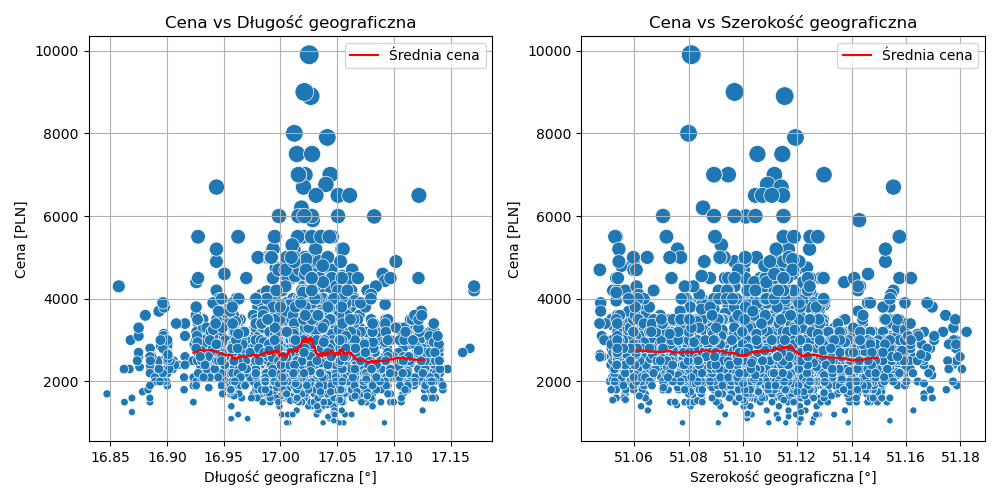
\includegraphics[width=0.8\textwidth]{coordinates-price.png}
    \caption{Wykres rozrzutu współrzędnych geograficznych i ceny wynajmu mieszkania z linią średniej ceny}
    \label{fig:coordinates_price}
\end{figure}


Analizując wykres \ref{fig:coordinates_price} można zauważyć, że zagęszczenie punktów jest największe w centrum miasta. 
Dlatego stworzono mapę ciepła opartą na jądrowym estymatorze gęstości(KDE) w celu dalszej analizy.
Jako parametr wygładzający estymatora wybrany został $ h = 0.3 $, ponieważ parametry $ h = 0.1 $ i $ h = 0.15 $ prowadziły do zbyt szczegółowej estymacji, 
a parametr $ h = 0.5 $ za bardzo uogólniał wynik.
Wartości wyjściowe zostały znormalizowane.
\begin{figure}[H]
    \centering
    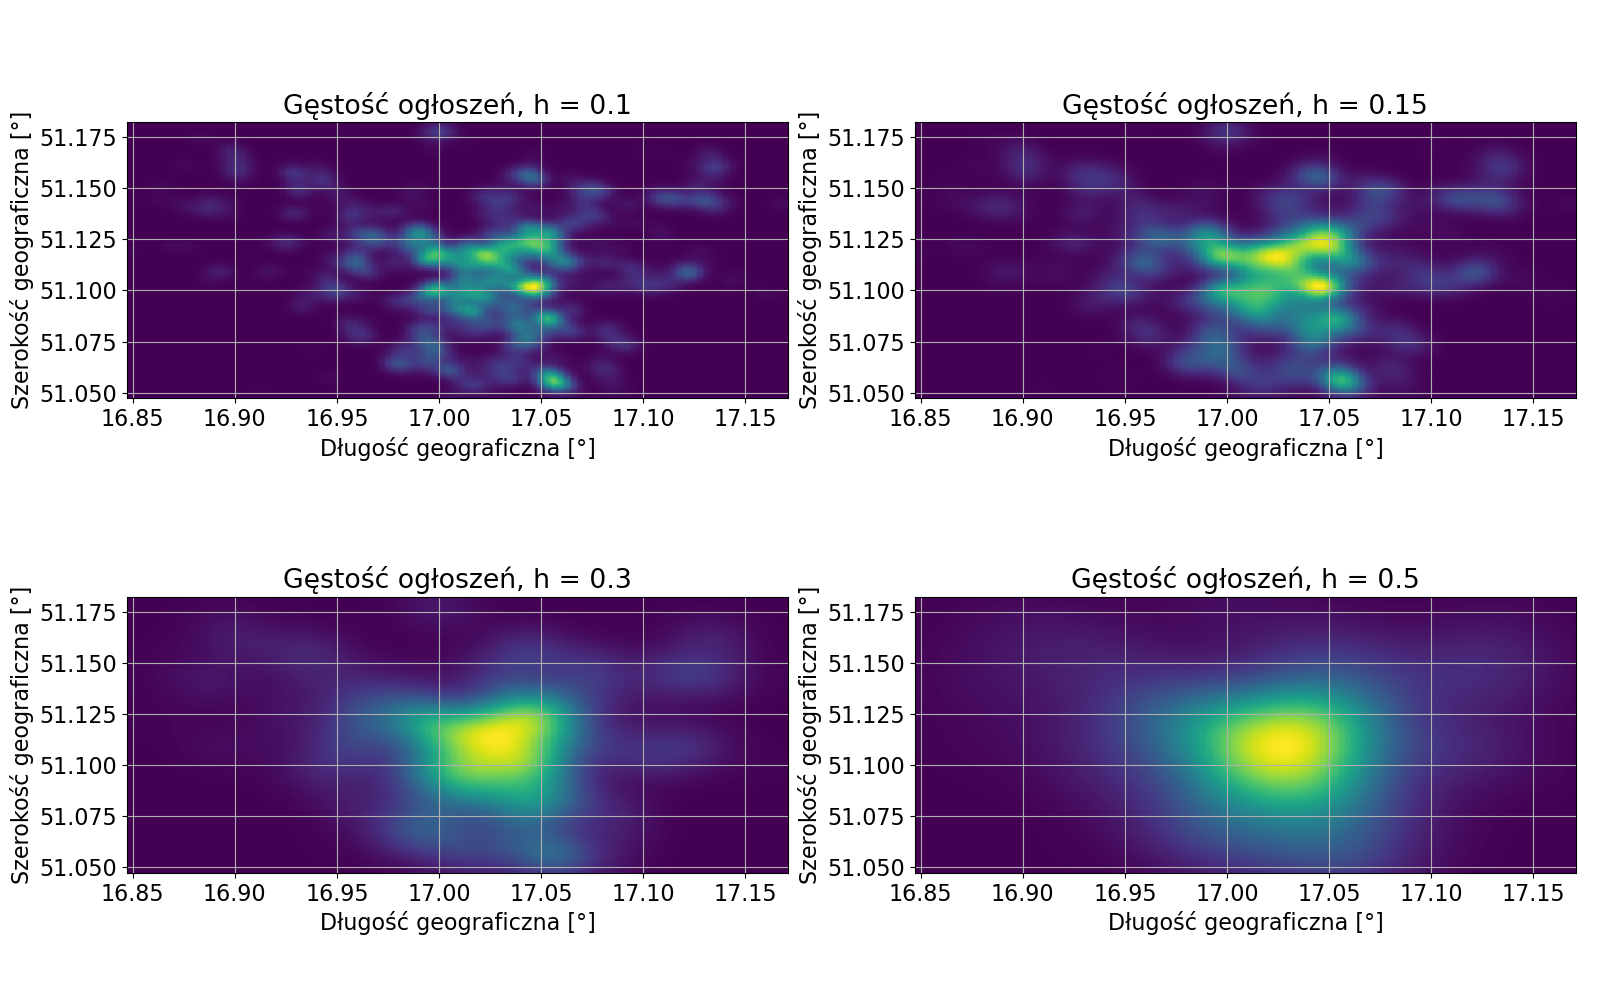
\includegraphics[width=0.8\textwidth]{kde-heatmap.png}
    \caption{Mapy ciepła szacowanej gęstości w zależności od parametru wygładzającego}
    \label{fig:kde_heatmap}
\end{figure}

Nakreślenie wykresu zależności ceny od gęstości ofert nie wykazuje dużego powiązania między tymi dwiema charakterystykami, co potwierdza współczynnik korelacji liniowej równy $ 0.09 $.

\begin{figure}[H]
    \centering
    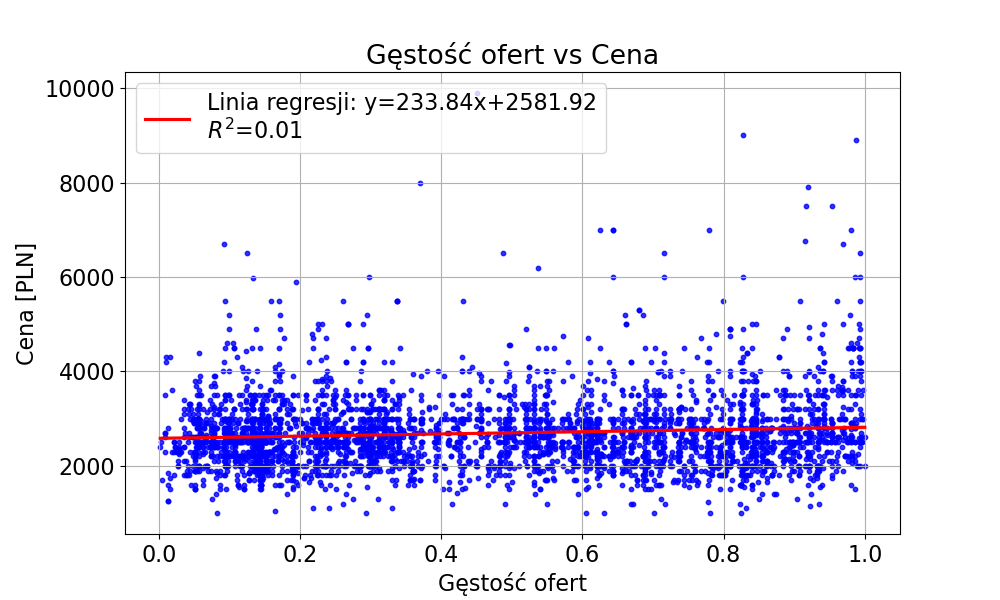
\includegraphics[width=0.6\textwidth]{density-price.png}
    \caption{Wykres rozrzutu gęstości ofert i ceny wynajmu mieszkania z linią regresji}
    \label{fig:density_price}
\end{figure}


Interesujące wyniki ukazują się po rozdzieleniu ofert mieszkań w zależności od rodzaju zabudowy i ponownym zbadaniu zależności ceny od gęstości ofert.
Analiza wykresów wskazuje na to, iż na cene mieszkania w bloku nie ma wpływu jego położenie. Podobna sytuacja ma miejsce dla kamienic.
Natomiast dla mieszkań typu apartamentowiec dostrzegalna jest delikatna korelacja lokalizacji mieszkania z ceną wynajmu.
Potwierdza to nieco lepszy współczynnik determinacji $ R^2 = 0.04 $ oraz zauważalnie lepszy współcznnik korelacji liniowej równy $ 0.19 $.
Podobny trend zdaje się być prawdziwy dla pozostałych rodzajów mieszkań. 
Jednak z uwagi na ich heterogeniczną naturę oraz małą liczbe danych ich dotyczących, nie można wykluczyć stronniczości ze strony zestawu danych.

\begin{figure}[H]
    \centering
    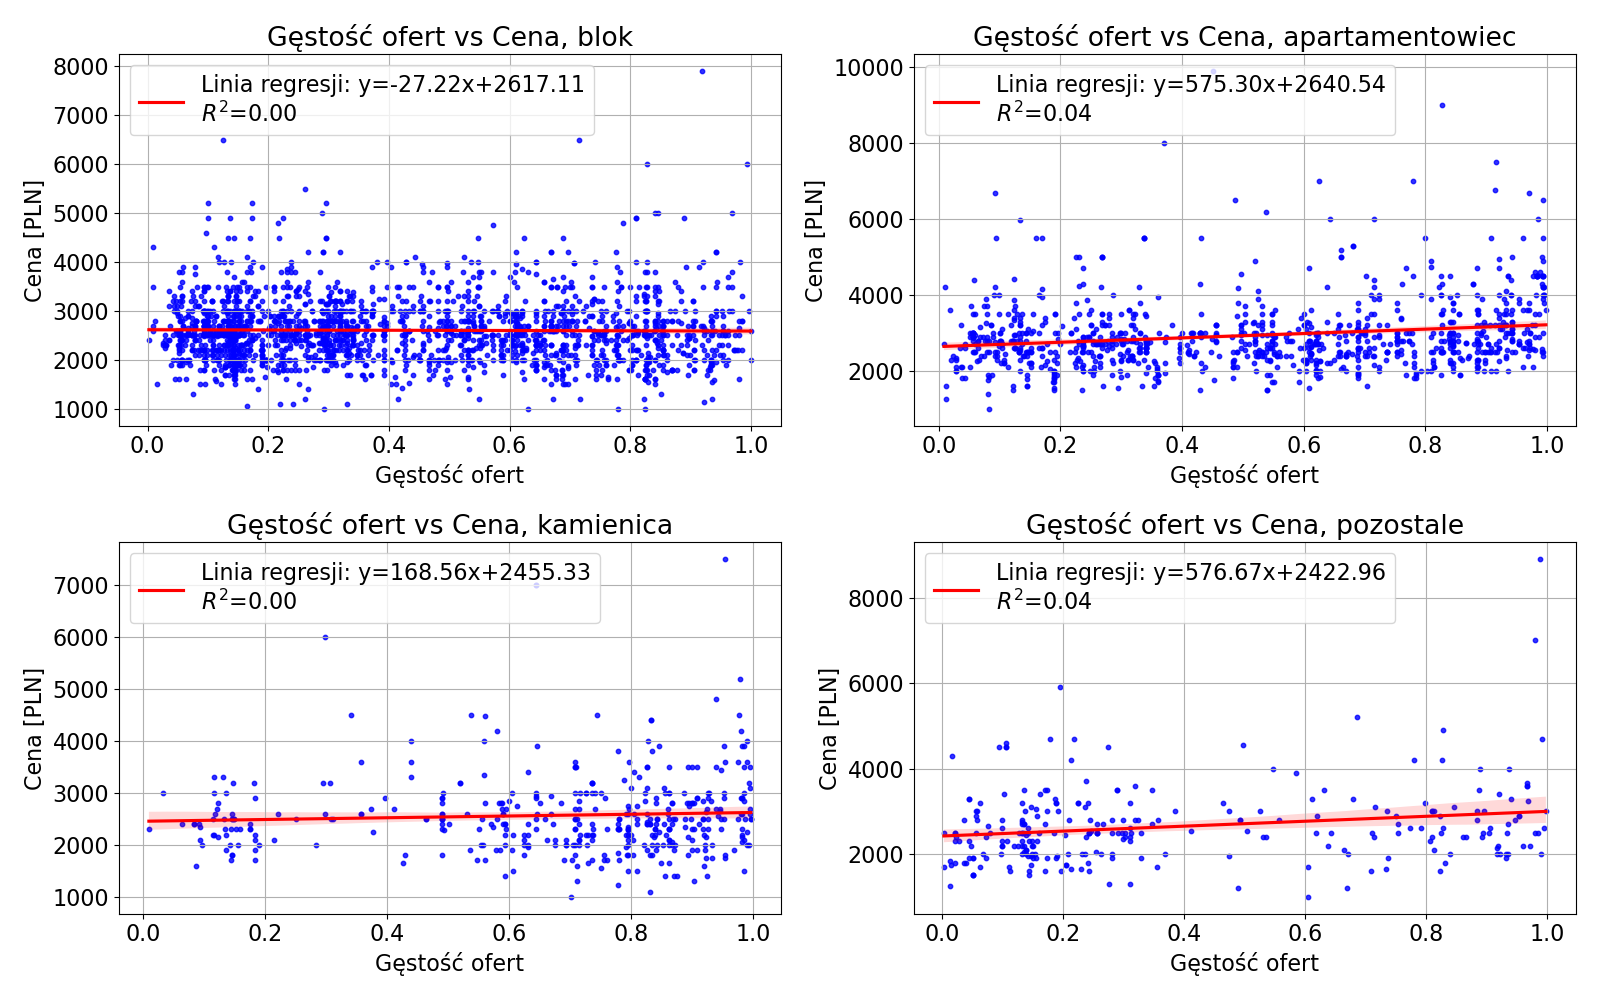
\includegraphics[width=0.8\textwidth]{density-price-builttype.png}
    \caption{Wykres rozrzutu gęstości ofert i ceny wynajmu mieszkania z linią regresji dla różnych rodzajów zabudowy}
    \label{fig:density_price_builttype}
\end{figure}


\subsection{Plan badań}
Na podstawie uprzednio zbadanych zależności w danych, sporządzone zostaną modele regresji liniowej, osobno dla każdego rodzaju zabudowy mieszkania.
Dla mieszkań typu apartamentowiec wykorzystane będą dane dot. metrażu i lokalizacji. Dla pozostałych, brane pod uwage będą tylko dane o powierzchni mieszkań.

Zbiór danych zostanie podzielony na dane trenujące i testowe w proporcji 80/20. Działanie modelu będzie ocenione na podstawie jego współczynnika determinacji $ R^2 $ oraz pierwiastka błędu średniokwadratowego (MSRE).
Dodatkowo w celu potwierdzenia czy informacja o lokalizacji pozytywnie wpływa na działanie estymatora, porównany zostanie model wykorzystujący je z modelem opartym wyłącznie o dane o metrażu mieszkania.

\section{Wyniki obliczeń}

\subsection{Blok}
Dla mieszkania w bloku model przyjął postać 
\begin {equation}
y = 32.45x + 1171.42
\end{equation}
gdzie y to szacowana cena wynajmu mieszkania, a x to jego powierzchnia.
Model osiągnął współczynnik determinacji $ R^2 = 0.55 $ i $ MSRP = 416.10 $.

\begin{figure}[H]
    \centering
    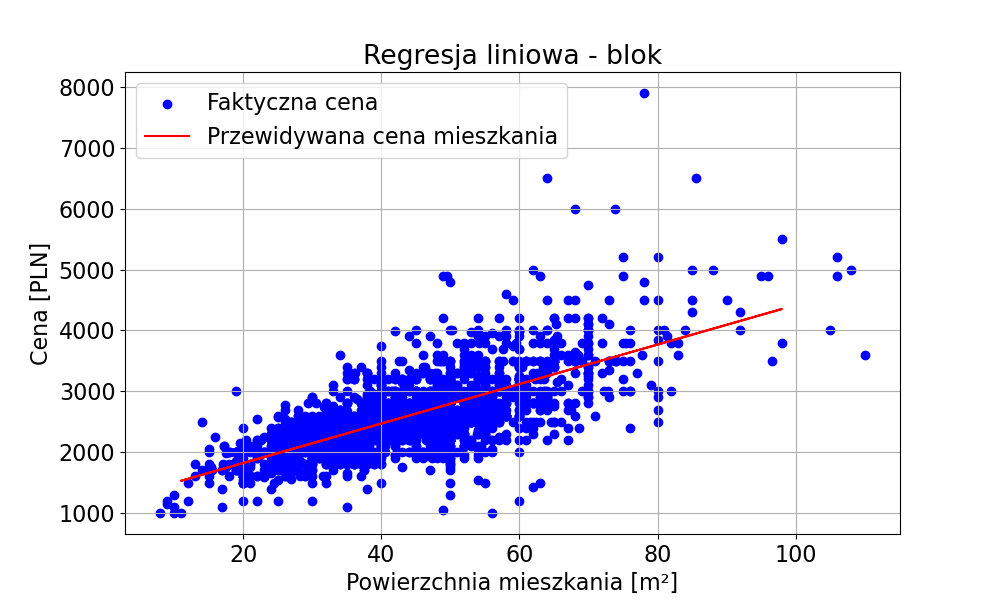
\includegraphics[width=0.6\textwidth]{regression-blok.png}
    \caption{Wykres rozrzutu ceny mieszkań w bloku i linia regresji modelu}
    \label{fig:regression-blok}
\end{figure}


\subsection{Apartamentowiec}
Dla mieszkania w apartentowcu model przyjął postać 
\begin {equation}
y = 46.88x + 612.41z + 594.91
\end{equation}

gdzie y to szacowana cena wynajmu mieszkania, a $ x $ to jego powierzchnia, a $ z $ to wartość funkcji gęstości.
Model osiągnął współczynnik determinacji $ R^2 = 0.65 $ i $ MSRP = 478.31 $.

Przy identycznym podzale danych treningowych, sporządzony został model wykorzystujący jedynie dane o powierzchni mieszkania i przyjął postać
\begin {equation}
y = 46.55x + 924.96
\end{equation}

Model osiągnął współczynnik determinacji $ R^2 = 0.58 $ i $ MSRP = 522.17 $.
Zatem dostrzegalny jest niewielki, ale realny wpływ położenia na cenę mieszkań w tym rodzaju zabudowy.

\begin{figure}[H]
    \centering
    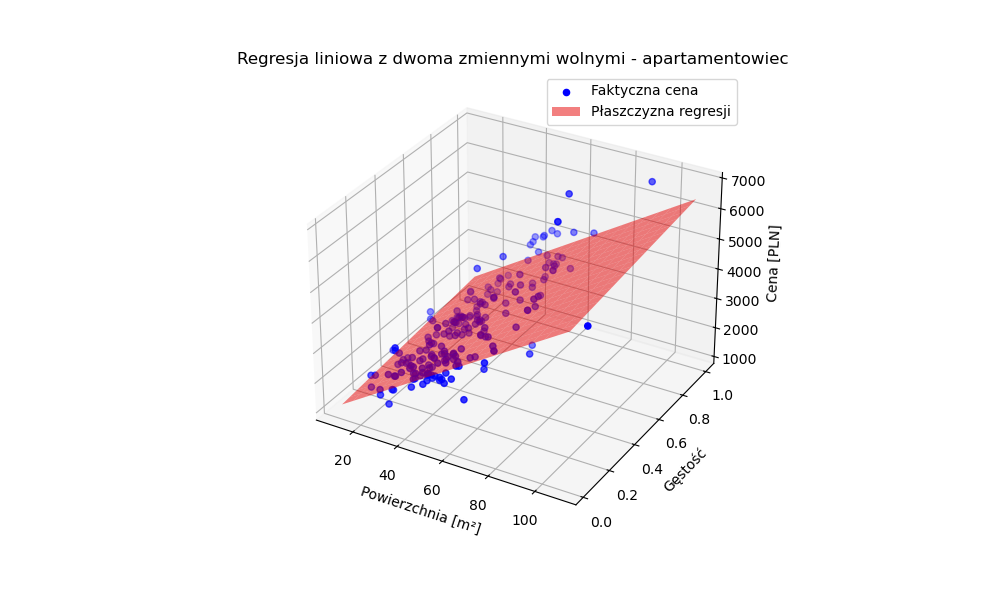
\includegraphics[width=0.8\textwidth]{regression-2d-apartamentowiec.png}
    \caption{Wykres rozrzutu ceny mieszkań w apartamentowcu i płaszczyzna regresji modelu}
    \label{fig:regression-2d-apartamentowiec}
\end{figure}



\subsection{Kamienica}
Dla mieszkania w kamienicy model przyjął postać 
\begin {equation}
y = 33.31x + 1092.13
\end{equation}
gdzie y to szacowana  wynajmu wynajmu mieszkania, a x to jego powierzchnia.
Model osiągnął współczynnik determinacji $ R^2 = 0.48 $ i $ MSRP = 535.02 $.

\begin{figure}[H]
    \centering
    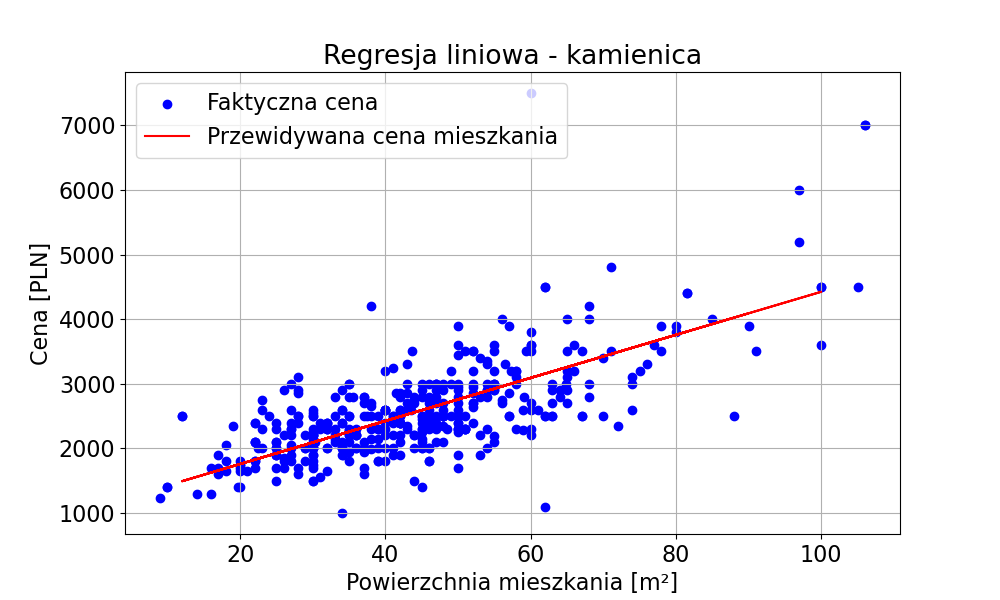
\includegraphics[width=0.6\textwidth]{regression-kamienica.png}
    \caption{Wykres rozrzutu ceny mieszkań w kamienicy i linia regresji modelu}
    \label{fig:regression-kamienica}
\end{figure}


\subsection{Pozostałe}
Dla mieszkania w pozostałych rodzajach zabudowy model przyjął postać 
\begin {equation}
y = 33.19x + 1119.37
\end{equation}
gdzie y to szacowana cena wynajmu mieszkania, a x to jego powierzchnia.
Model osiągnął współczynnik determinacji $ R^2 = 0.44 $ i $ MSRP = 595.53 $.

\begin{figure}[H]
    \centering
    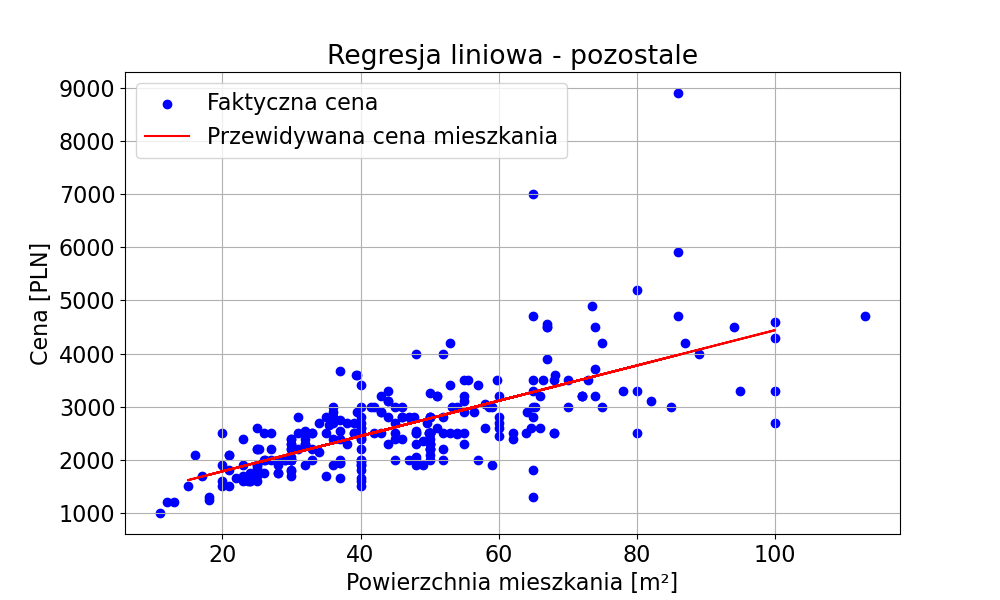
\includegraphics[width=0.6\textwidth]{regression-pozostale.png}
    \caption{Wykres rozrzutu ceny mieszkań w pozostałych rodzajach zabudowy i linia regresji modelu}
    \label{fig:regression-pozostale}
\end{figure}


\section{Wnioski}
Przewidywanie cen wynajmu mieszkań we Wrocławiu jest nietrywialnym zadaniem.
Jest to szczególnie trudne bez szczegółowych charakterystyk dot. mieszkania jak na przykład jakościowe oznaczenie nieruchomości, 
które ciężko jest obiektywnie ocenić, a tym bardziej z parametrów podanych na serwisie ogłoszeniowym bez analizy zdjęć.
W pewnym sensie rodzaj zabudowy oddaje do pewnego stopnia jakość mieszkania, chociaż dokładniejsze dane na pewno pozytywnie wpłynełyby na jakość modeli.

Dodatkowym czynnikiem niekorzystnym dla modelowania tego wycinka rzeczywistości może być nieatrakcyjna gospodarka nieruchomości w mieście, 
która może powodować duże rozbieżności w cenach mieszkań spowodowane zawyżaniem cen mieszkań a co za idzie kosztów wynajmu.

Modele cen mieszkań w bloku i apartamentowcu przyniosły najlepsze odwzorowanie, możliwe, że jest to spowodowane dużą ilością danych zgromadzonych na temat tego rodzaju mieszkań.
Istnieje nadal miejsce do ulepszenia modeli, chociażby poprzez zgromadzenie większej ilości danych na temat mniej popularnych rodzajów mieszkań lub przez znalezienie nowej zmiennej niezależnej. 


Ciekawym faktem jest, że lokalizacja nie ma niemalże żadnego wpływu na koszt wynajmu mieszkania w bloku, 
co prawdopodobnie powiązane jest z wcześniej wspomnianą sytuacją na rynku nieruchomości.
Dlatego prawdopodobnie ludzie przy wyborze mieszkania wybierają takie które jest dostępne, a mieszkań w bloku jest najwięcej.


\newpage


\appendix
\section{Dodatek}
Kody źródłowe umieszczone zostały w repozytorium github:

\noindent \url{https://github.com/b0czek/msid-raport}.


\end{document}
